\documentclass{article}
% 这里是导言区
%\usepackage{indentfirst}%缩进控制
\usepackage{listings}%插入代码
\usepackage{mcode}
%ctex能够保证能够渲染英文
\usepackage{ctex}
\usepackage{textcomp}
\usepackage{graphicx}%插入图像
\usepackage{epstopdf}
\usepackage{amsmath}
\usepackage{graphicx}
\usepackage{subfigure}
\usepackage{geometry}%设置页边距
\usepackage{amssymb}
\usepackage{float}
\usepackage[level]{datetime} 
\makeatletter
\newcommand{\rmnum}[1]{\romannumeral #1}
\newcommand{\Rmnum}[1]{\expandafter\@slowromancap\romannumeral #1@}
\makeatother
% \renewcommand\thesection{\roman{subsection}}
%\newdateformat{ukdate}{\ordinaldate{\THEDAY} \monthname[\THEMONTH]

\geometry{a4paper,scale=0.75}


\lstset{
tabsize=4, %tab 空格数
frame=shadowbox, %把代码用带有阴影的框圈起来
rulesepcolor=\color{red!20!green!20!blue!20}, %代码块边框为淡青色
keywordstyle=\color{blue!90}\bfseries, %代码关键字的颜色为蓝色, 粗体
showstringspaces=false, %不显示代码字符串中间的空格标记
stringstyle=\ttfamily, %代码字符串的特殊格式
keepspaces=true, %
breakindent=22pt, %
numbers=left, %左侧显示行号
stepnumber=1, %
numberstyle=\tiny, %行号字体用小号
basicstyle=\footnotesize, %
showspaces=false, %
flexiblecolumns=true, %
breaklines=true, %对过长的代码自动换行
breakautoindent=true, %
breakindent=4em, %
aboveskip=1em, %代码块边框
}

\title{Chapter3}
\author{31202008881        \quad \quad \quad
          Bao Ze an}

\begin{document}
\setlength{\parindent}{0em}
\maketitle

\section*{3.1}
\par
\centerline{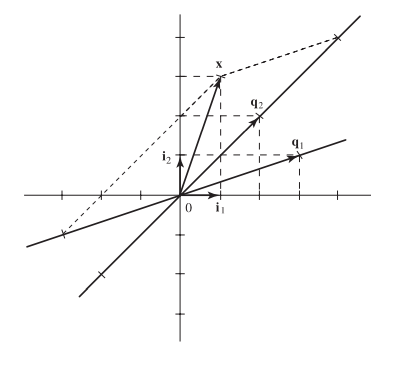
\includegraphics[width = .8\textwidth]{a3.1.PNG}}
\centerline
\par
From the above figure, The three vectors $\boldsymbol{q}_{1}=\left[\begin{array}{ll}3 & 1\end{array}\right]^{\prime}, \boldsymbol{i}_{2}=\left[\begin{array}{ll}0 & 1\end{array}\right]^{\prime}$ and $\boldsymbol{q}_{2}=\left[\begin{array}{ll}2 & 2\end{array}\right]^{\prime}$\\
The representation of $x$ with respect to $\left\{\boldsymbol{q}_{1}, \boldsymbol{i}_{2}\right\}$ is $\left[\begin{array}{ll}\frac{1}{3} & \frac{8}{3}\end{array}\right]^{\prime}$\\
The representation of $\boldsymbol{q}_{1}$ with respect to $\left\{\boldsymbol{i}_{2}, \boldsymbol{q}_{2}\right\}$ is $\left[\begin{array}{ll}-2 & \frac{3}{2}\end{array}\right]^{\prime}$\\
These can be verified like this:
$$
x=\left[\begin{array}{l}
1 \\
3
\end{array}\right]=\left[\begin{array}{ll}
\boldsymbol{q}_{1} & \boldsymbol{i}_{2}
\end{array}\right]\left[\begin{array}{l}
\frac{1}{3} \\
\frac{8}{3}
\end{array}\right]=\left[\begin{array}{ll}
3 & 0 \\
1 & 1
\end{array}\right]\left[\begin{array}{l}
\frac{1}{3} \\
\frac{8}{3}
\end{array}\right]
$$
\section*{3.2}
\subsection*{\rmnum{1}:The norm of $x_{1}$}
1-norm: $\left\|x_{1}\right\|_{1}=\sum_{i=1}^{3}\left|x_{i}\right|=|2|+|-3|+|1|=6$\\
2 -norm: $\left\|\boldsymbol{x}_{1}\right\|_{2}=\left(\sum_{i=1}^{3}\left|x_{i}\right|^{2}\right)^{\frac{1}{2}}=\sqrt{2^{2}+|-3|^{2}+1^{2}}=\sqrt{14}$\\
infinite-norm: $\left\|\boldsymbol{x}_{1}\right\|_{\infty}=\max _{i}\left|x_{i}\right|=3$\\\
\subsection*{\rmnum{2}:The norm of $x_{2}$}
1 -norm: $\left\|\boldsymbol{x}_{2}\right\|_{1}=\sum_{i=1}^{3}\left|x_{i}\right|=|1|+|1|+|1|=3$\\
2-norm: $\left\|\boldsymbol{x}_{2}\right\|_{2}=\left(\sum_{i=1}^{3}\left|x_{i}\right|^{2}\right)^{\frac{1}{2}}=\sqrt{1^{2}+1^{2}+1^{2}}=\sqrt{3}$\\
infinite-norm: $\left\|\boldsymbol{x}_{2}\right\|_{\infty}=\max _{i}\left|x_{i}\right|=1$\\

\section*{3.3}
This is just the orthonormalization procedure.
$$
\left\{\begin{array}{ll}
u_{1}=\alpha_{1} & q_{1}=u_{1} /\left\|u_{1}\right\| \\
u_{2}=\alpha_{2}-\left(q_{1}^{\prime} \alpha_{2}\right) q_{1} & q_{2}=u_{2} /\left\|u_{2}\right\|
\end{array}\right.
$$
This is the ordinary method,what we find is the two vector are orthogonal. so,we just need to make the length of vector is 1 .
$$
\begin{array}{c}
q_{1}=\frac{u_{1}}{\left\|u_{1}\right\|}=\left[\frac{2}{\sqrt{14}}-\frac{3}{\sqrt{14}} \quad \frac{1}{\sqrt{14}}\right]^{\prime} \\
q_{1}=\frac{u_{2}}{\left\|u_{2}\right\|}=\left[\frac{1}{\sqrt{3}} \quad \frac{1}{\sqrt{3}} \quad \frac{1}{\sqrt{3}}\right]^{\prime}
\end{array}
$$

\section*{3.4}
\subsection*{a}
if n>m,$\boldsymbol{AA}^{'}$ is a ordinary vector,which has the rank m\\
\subsection*{b}
if m=n,so $\boldsymbol{A}$ is a nonsingular square matrix,we already have $\boldsymbol{A}^{'}\boldsymbol{A}=\boldsymbol{I}_m$,so $\boldsymbol{A}'=\boldsymbol{A}^{-1}$.
$\boldsymbol{AA}^{'}=\boldsymbol{A}\boldsymbol{A}^{-1}=\boldsymbol{I}_n$

\section*{3.5}
Accoridng to the principle:\\
\[Nillity(\boldsymbol{A})=number of columns of \boldsymbol{A}-rank\boldsymbol(A)\]
\subsection*{\rmnum{1}:}
Rank $\boldsymbol(A_1)=2$\\
Nullity $\boldsymbol(A_1)=3-2=1$
\subsection*{\rmnum{2}:}
Rank $\boldsymbol(A_2)=3$\\
Nullity $\boldsymbol(A_2)=3-3=0$\\
\subsection*{\rmnum{3}:}
Rank $\boldsymbol(A_3)=3$\\
Nullity $\boldsymbol(A_3)=4-3$

\section*{3.6}
For $A_1$:
\begin{equation*}
\boldsymbol{a_1}=
\left[
\begin{array}{c}
1\\
0\\
0
\end{array}
\right]
\boldsymbol{a_2}=
\left[
\begin{array}{c}
0\\
0\\
1\\
\end{array}
\right]
\end{equation*}
The set of $\{\boldsymbol{a_1},\boldsymbol{a_2}\}$ can be the basis of the range spaces.\\
The independent vectors of null space can get by solving the equation:\\
\[\boldsymbol{A}_1 \boldsymbol{\eta}_i=0\]
\begin{equation*}
\boldsymbol{\eta}_1=
\left[
\begin{array}{c}
1\\
0\\
0\\
\end{array}
\right]
\end{equation*}
The set of ${\boldsymbol{\eta}_1}$ is the basis of the null space\\
in the same way,we can get the basis of the range space and null space of $\boldsymbol{A}_2$
\begin{equation*}
\boldsymbol{a_1}=
\left[
\begin{array}{c}
4\\
3\\
1
\end{array}
\right]
\boldsymbol{a_2}=
\left[
\begin{array}{c}
1\\
2\\
1\\
\end{array}
\right]
\boldsymbol{a_3}=
\left[
\begin{array}{c}
-1\\
0\\
0\\
\end{array}
\right]
\end{equation*}
The set of  $\{\boldsymbol{a_1},\boldsymbol{a_2},\boldsymbol{a_3}\}$ is the basis of the range space.\\
because the $\boldsymbol{A}_2$ is full rank,so the basis of the null space is $\{\boldsymbol{0}\}$

\section*{3.7}
\[\rho(\boldsymbol{A})=\rho([\boldsymbol{A}\quad y])=2\]
so a solution $\boldsymbol{x}$ exist with respect to this equation.\\
Because coefficient matrix is full column rank,so the solution is unique.\\
if y=$[1\quad 1\quad 1]^{'}$,$\rho(\boldsymbol{A})=2 \neq \rho([\boldsymbol{A}\quad y])=3$
so,when $\boldsymbol{y}$=$[1 \quad 1\quad 1]^{'}$,the solution is not exist.

\section*{3.8}
$\boldsymbol{x}_p=[0\quad -2\quad 1\quad 1]^{'}$ is a solution, a basis of the null space of $A$:
\[\boldsymbol{A} \boldsymbol{\eta}_i=0\]
\begin{equation*}
\boldsymbol{\eta}_1=
\left[
\begin{array}{c}
1\\
-2\\
1\\
0\\
\end{array}
\right]
\end{equation*}
Thus the gengeral solution can be expressed as:
\[\boldsymbol{x}=\boldsymbol{x}_p+\alpha_1 \boldsymbol{\eta}_1\]

\section*{3.9}
From the example 3.3,we can know the gengeral solution is:
\begin{equation*}
\boldsymbol{x}=
\left[
\begin{array}{c}
\alpha_1\\
-4+\alpha_1+2\alpha_2\\
-\alpha_1\\
-\alpha_2
\end{array}
\right]
\end{equation*}
\[\left\|\boldsymbol{x}\right\|_2=\sqrt{\alpha_1^2+(\alpha_1+2*\alpha_2-4)^2+\alpha_1^2+\alpha_2^2}\]
adjusting polynomials into sum of squares:
\[\sqrt{3(\alpha_1+\frac{2}{3}(\alpha_2-2))^2+\frac{11}{3}(\alpha_2-\frac{16}{11})^2+\frac{32}{11}-(\frac{16}{11})^2}\]
When all the square terms are zero, the Euclidean norm of the solution is the smallest
so,we can get
\[
\left\{
\begin{aligned}
&\alpha_1=\frac{4}{11}& \\   
&\alpha_2=\frac{16}{11}&
\end{aligned}
\right.
\]
so the solution,which can get the smallest Euclidean is :
\begin{equation*}
\boldsymbol{x}=
\left[
\begin{array}{c}
\frac{4}{11}\\
-\frac{8}{11}\\
-\frac{4}{11}\\
-\frac{16}{11}
\end{array}
\right]
\end{equation*}

\section*{3.9}
In the same way as in the problem 3.9,but we can find the extremum by derivation
\begin{equation*}
\boldsymbol{x}=
\left[
\begin{array}{c}
\alpha_1\\
-2-\alpha_1\\
1+\alpha_1\\
1
\end{array}
\right]
\end{equation*}
\[\left\|\boldsymbol{x}\right\|_2^2=6\alpha_1^2+10\alpha+6\]
\[\dot{\left\|\boldsymbol{x}\right\|_2^2}=12\alpha_1+10=0\]
\[\alpha_1=-\frac{5}{6}\]
so the solution,which have the smallest Euclidean is:
\begin{equation*}
\boldsymbol{x}=
\left[
\begin{array}{r}
-\frac{5}{6}\\
-\frac{1}{3}\\
\frac{1}{6}\\
1
\end{array}
\right]
\end{equation*}

\section*{3.11}
There will exist $u[0],u[1],...,u[n-1]$ to meet the equation
for any x[n] and x[0],which means for any x[n] and x[0],the equation
is always have the solution,so $\boldsymbol{b},\boldsymbol{Ab},...,\boldsymbol{A^{n-1}b}$ must be linearly indepedent


\section*{3.12}
\begin{equation*}
\boldsymbol{b}=
\left[
\begin{array}{c}
0\\
0\\
1\\
1\\
\end{array}
\right]
\boldsymbol{Ab}=
\left[
\begin{array}{c}
0\\
1\\
2\\
1\\
\end{array}
\right]
\boldsymbol{A^2b}=
\left[
\begin{array}{c}
1\\
4\\
4\\
1\\
\end{array}
\right]
\boldsymbol{A^3b}=
\left[
\begin{array}{c}
6\\
12\\
8\\
1\\
\end{array}
\right]
\end{equation*}
Thus the representation of $A$ with respect to the basis {$\boldsymbol{b},\boldsymbol{Ab},\boldsymbol{A^2b},\boldsymbol{A^3b}$} is 
\begin{equation*}       %开始数学环境
\overline{A}=
\left[                %左括号
\begin{array}{cccc}   %该矩阵一共3列,每一列都居中放置
0& 0 &0 & 0\\  %第一行元素
1 & 0 &0 &20\\
0 & 1& 0 &-18 \\  
0 & 0 & 1& 7
\end{array}
\right]
\end{equation*}
The other basis:
\begin{equation*}
\boldsymbol{b}=
\left[
\begin{array}{c}
1\\
2\\
3\\
1\\
\end{array}
\right]
\boldsymbol{Ab}=
\left[
\begin{array}{c}
4\\
7\\
6\\
1\\
\end{array}
\right]
\boldsymbol{A^2b}=
\left[
\begin{array}{c}
15\\
20\\
12\\
1\\
\end{array}
\right]
\boldsymbol{A^3b}=
\left[
\begin{array}{c}
50\\
52\\
24\\
1\\
\end{array}
\right]
\end{equation*}
the representation of $A$ with respect to the basis {$\boldsymbol{\overline{b}},\boldsymbol{A\overline{b}},\boldsymbol{A^2overline{b}},\boldsymbol{A^3\overline{b}}$}
is the same as above.
\section*{3.13}
The Jordan-form representation of the matrices respectively is:$\hat{A}_{1},\hat{A}_{2},\hat{A}_{3},\hat{A}_{4}$
\begin{equation*}
\hat{A}_{1}=\left[\begin{array}{lll}
1 & 0 & 0 \\
0 & 2 & 0 \\
0 & 0 & 3
\end{array}\right]
\hat{A}_{2}=\left[\begin{array}{ccc}
    -1 & 0 & 0 \\
    0 & -1+j & 0 \\
    0 & 0 & -1-j
    \end{array}\right]
\hat{A}_{3}=\left[\begin{array}{lll}
    1 & 0 & 0 \\
    0 & 1 & 0 \\
    0 & 0 & 2
    \end{array}\right]
\hat{A}_{3}=\left[\begin{array}{lll}
    0 & 0 & 0 \\
    0 & 0 & 1 \\
    0 & 0 & 0
    \end{array}\right]
\end{equation*}
Because $A_4$ can not be diagonalized,so we calculate the $Q$,
which meets $Q^{-1}A_4Q=\hat{A}_{4}$\\
from the definition:
$$
\left\{\begin{array}{ll}
\boldsymbol{Av_1}=\lambda\boldsymbol{v_1}\\
\boldsymbol{Av_2}=\lambda\boldsymbol{v_2}+\boldsymbol{v_1}\\
\boldsymbol{Av_3}=\lambda\boldsymbol{v_3}+\boldsymbol{v_2}\\
\end{array}\right.
$$
we can calculate :
\begin{equation*}
\boldsymbol{v_1}=
\left[
\begin{array}{c}
1\\
0\\
0\\
\end{array}
\right]
\boldsymbol{v_2}=
\left[
\begin{array}{c}
1\\
-4\\
5\\
\end{array}
\right]
\boldsymbol{v_3}=
\left[
\begin{array}{c}
1\\
-7\\
9\\
\end{array}
\right]
\end{equation*}
\[\boldsymbol{Q}=[\boldsymbol{v_1,v_2,v_3}]\]

\section*{3.14}
The characteristic polynomial of $\delta(\lambda)=|\lambda E-A|$
\[|\lambda E-A|=
\left|
\begin{array}{cccc}
\lambda+\alpha_1 & \lambda_2 &\lambda_3 & \lambda_4\\
-1 & \lambda & 0 & 0\\
0 & -1 & \lambda & 0\\
0 & 0 & -1 & \lambda\\
\end{array}\right|
=\lambda^4+\alpha_1\lambda^3+\alpha_2\lambda^2+\alpha_3\lambda+\alpha_4
\]
for $\alpha=[\lambda_i^3 \quad \lambda_i^2 \quad \lambda_i \quad 1]^{'}$
we can vertify that $(\lambda_iE-A)\alpha=0$\\
so $\alpha=[\lambda_i^3 \quad \lambda_i^2 \quad \lambda_i \quad 1]^{'} $ is an eigenvector of A associated with $\lambda_i$.

\section*{3.15}
\[
\left|
\begin{array}{cccc}
\lambda_1^3 & \lambda_2^3 & \lambda_3^3 & \lambda_4^3\\
\lambda_1^2 & \lambda_2^2 & \lambda_3^2 & \lambda_4^2\\
\lambda_1 & \lambda_2 & \lambda_3 & \lambda_4\\
\end{array}\right|
=
\left|
\begin{array}{cccc}
0 & \lambda_2^3-\lambda_1\lambda_2^2 & \lambda_3^3-\lambda_1\lambda_3^2 & \lambda_4^3-\lambda_1\lambda_4^2\\
0 & \lambda_2^2-\lambda_1\lambda_2 & \lambda_3^2-\lambda_1\lambda_3 & \lambda_4^2-\lambda_1\lambda_4\\
0 & \lambda_2-\lambda_1 & \lambda_3-\lambda_1 & \lambda_4-\lambda_1\\
\end{array}\right|
=(\lambda_2-\lambda_1)(\lambda_3-\lambda_1)(\lambda_4-\lambda_1)
\left|
\begin{array}{ccc}
\lambda_2^2 & \lambda_3^2 & \lambda_4^2\\
\lambda_2 & \lambda_3 & \lambda_4\\
1 & 1 &1\\
\end{array}
\right|
\]
\[=\prod \limits_{1 \leq i < j \leq 4}(\lambda_j-\lambda_i)\]

\section*{3.16}
\[|\boldsymbol{A}|
=
\left|
\begin{array}{cccc}
-\alpha_1 & -\alpha_2 & -\alpha_3 & -\alpha_4\\
1 & 0 & 0 &0\\
0 & 1 & 0 &0\\
0& 0 &1 &0
\end{array}
\right|
\]
so,when $\alpha_4 \neq 0$,the companion-form matrix is nonsingular,\\
when the matrix is nonsingular,so matrix A can inverse.\\
\[\boldsymbol{AA^{-1}=A^{-1}A=E}\]

\section*{3.17}
\[
(\boldsymbol{A}-\lambda\boldsymbol{I})^3=
\left[
\begin{array}{ccc}
0 & 0 & 0\\
0 & 0 & 0\\
0 & 0 & 0\\
\end{array}
\right]
\quad
(\boldsymbol{A}-\lambda\boldsymbol{I})^2=
\left[
\begin{array}{ccc}
0 & 0 & \lambda^2T^2\\
0 & 0 &0\\
0 & 0 &0\\
\end{array}
\right]
\]
For $v=[0 \quad 0 \quad 1]^{\prime}$,we can vertify $(\boldsymbol{A}-\lambda\boldsymbol{I})^3\boldsymbol{v}=\boldsymbol{0}$,$(\boldsymbol{A}-\lambda\boldsymbol{I})^2\boldsymbol{v} \neq \boldsymbol{0}$\\
so from the definition,we can say $[0 \quad 0 \quad 1]^{\prime}$ is a generalized eigenvector of grade 3.\\
\[
\boldsymbol{v_1}=
\left[
\begin{array}{c}
\lambda^2T^2\\
0\\
0\\
\end{array}
\right]   
\boldsymbol{v_2}=
\left[
\begin{array}{c}
\lambda T^2\\
\lambda T\\
0
\end{array}
\right]
\boldsymbol{v_3}=
\left[
\begin{array}{c}
0\\
0\\
1\\
\end{array}
\right]
\]
we can vertify that 
\[
\left\{
\begin{aligned}
&\boldsymbol{Av_1}=\lambda\boldsymbol{v_1}&\\
&\boldsymbol{Av_2}=\lambda\boldsymbol{v_2}+\boldsymbol{v_1}&\\
&\boldsymbol{Av_3}=\lambda\boldsymbol{v_3}+\boldsymbol{v_2}&\\
\end{aligned}
\right.
\]
so the three columns of $Q$ constitute a chain of generalized eigenvectors of length 3.\\
It is also easy to vertify that 
\[Q^{-1}AQ=
\left[
\begin{array}{ccc}
\lambda & 1 & 0\\
0 & \lambda & 1\\
0 & 0 & \lambda\\
\end{array}
\right]
\]

\section*{3.18}
The characteristic polynomials of $A,B,C,D$(from left to right) is 
$(\lambda-\lambda_1)^3(\lambda-\lambda_2)$,$(\lambda-\lambda_1)^4$,$(\lambda-\lambda_1)^4$,$(\lambda-\lambda_1)^4$
resepectively.\\

The minimal polynomials of $A,B,C,D$(from left to right)is
$(\lambda-\lambda_1)^3(\lambda-\lambda_2)$,$(\lambda-\lambda_1)^3$,$(\lambda-\lambda_1)^2$,$(\lambda-\lambda_1)$
resepectively.

\section*{3.19}
Because:$\boldsymbol{Ax}=\lambda x$,we have $\boldsymbol{A^kx}=\lambda^k\boldsymbol{x}$\\

without loss of generality,we specify that:$f(\lambda)=a_n\lambda^n+a_{n-1}\lambda^{n-1}+...+a_0$\\

so,for:
\[f(\boldsymbol{A}) \boldsymbol{x}=
a_n \boldsymbol{A^nx}+a_{n-1} \boldsymbol{A^{n-1}x}+\cdots+a_0 \boldsymbol{x}
=\\
(a_n\lambda^n+a_{n-1}\lambda^{n-1}+\cdots+a_0)x
=f(\lambda)x\]

so, $f(\lambda)$ is an eigenvector of $f(\boldsymbol{A})$ with the same eigenvector x.

\section*{3.20}
There exists a nonsingular matrix $Q$ made $Q^{-1}AQ=\hat{J}$,
where $\hat{J}$ is a Jordan form.If $A$ has any nonzero eigenvalues,then $A^k \neq 0$ for all interger k.\\
so,when $A^{k}=0$, we can conclude that its all eigenvalues must be zero.Thus to say,A has eigenvalues 0 with multiplicity n.
Let $\hat{J}=diag\{\hat{J}_1,\hat{J}_2,\cdots\}$,then $\hat{J}^{k}=diag\{\hat{J}^k_1,\hat{J}^k_2,\cdots\}.$
each $\hat{J}_i$ is a Jordan block associated with eigenvalue 0.then,we can obtain from(3.40) that $\boldsymbol{A}_i^m=\boldmath{0}$
where the m is the largest order of all Jordan blocks,so for $k \geq m$,we have $\boldsymbol{A}_i^k=\boldsymbol{0}$.
so $\boldsymbol{A}^k=\boldsymbol{0}$

\section*{3.21}
First,calculating the eigenvalues of the $A$:
\[
|\lambda E-A|=
\left|
\begin{array}{ccc}
\lambda-1 & -1 & 0\\
0 & \lambda & -1\\
0 & 0 & \lambda-1\\
\end{array}
\right|=
(\lambda-1)^2\lambda=0
\]
in this question,I want to use a complex method .
so, the eigenvalues are $\lambda_1=0,\lambda_2=\lambda_3=1$\\
for $\lambda_2=\lambda_3=1$,rank(E-A)=2,so,for eigenvalue 1,it dosen't have two indepedent eigenvectors,so there exists a nonsingular matrix $Q$ made the 
$Q^{-1}AQ=\hat{J}$,where $\hat{J}$ is a Jordan form .\\
from $Ax_1=x_1$,we can calculate a $x_1=[1 \quad 0 \quad 0]^{\prime}$\\
form $Ax_2=x_2+x_1$,we can calculate the $x_2=[1 \quad 1 \quad 1]^{\prime}$\\
from $Ax=0$,we can calculate a $x=[1 \quad -1 \quad 0]^{\prime}$\\
so for $Q=[x,x_1,x_2]$,we have 
\[Q^{-1}AQ=J=
\left[
\begin{array}{ccc}
0 & 0 &0\\
0 & 1 &1\\
0 & 0 &1\\
\end{array}
\right]
\]
we can split matrxi $J$ into $B$ and $C$,where:
\[
B=
\left[
\begin{array}{ccc}
0 & 0 & 0\\
0 & 1 & 0\\
0 & 0 & 1\\
\end{array}    
\right]
C=
\left[
\begin{array}{ccc}
0 & 0 & 0\\
0 & 0 & 1\\
0 & 0 & 0\\
\end{array}    
\right]
\]
\[J=B+C\]
\[A^{10}=QJ^{10}Q^{-1}=Q(B+C)^{10}Q^{-1}=Q(B^{10}+C^1_{10}B^9C)Q^{-1}=
\left[
\begin{array}{ccc}
1 & 1 &9\\
0 & 0 &1\\
0 & 0 &1\\
\end{array}
\right]
\]
in the same way,we can get:
\[
A^{103}=
\left[
\begin{array}{ccc}
1 & 1 & 102\\
0 & 0 & 1\\
0 & 0 & 1\\
\end{array}
\right]    
\]
from $f(\hat{J})=Q^{-1}f(A)Q$ and from (3.48) we can readily know:
\[e^{\hat{J}t}=
\left[
\begin{array}{ccc}
1 & 0 & 0\\
0 &e^{t} & te^{t}\\
0 & 0 & e^{t}\\
\end{array}
\right]
\] 
so 
\[e^{At}=Qe^{\hat{J}t}Q^{-1}
=\left[
\begin{array}{ccc}
e^t & e^t-1 & te^t-e^t+1\\
0 & 1 & e^t-1\\
0 & 0 & e^t\\   
\end{array}
\right]
\]

\section*{3.22}
\[
A_1=
\left[
\begin{array}{ccc}
1 & 4 & 10\\
0 & 2 & 0\\
0 & 0 &3\\   
\end{array}
\right]
A_4=
\left[
\begin{array}{ccc}
0 & 4 &3\\
0 & 20 & 16\\
0 & -25 &-20\\
\end{array}
\right]
\]

First method:$f(A)=h(A)$\\
for $A_1$,define $h(\lambda)=\beta+\beta_1\lambda+\beta_2\lambda^2$,$f(\lambda)=e^{\lambda t}$
from the problem3.13,the eigenvalues of the $A_1$ are 1,2,3\\
\[
\left\{
\begin{aligned}
&f(1)=h(1)&\\
&f(2)=h(2)&\\
&f(3)=h(3)&\\
\end{aligned}
\right.
\]
we can calculate that:
\[
\left\{
\begin{aligned}
&\beta_0=3e^t-3e^{2t}+e{3t}&\\
&\beta_1=-2.5e^t+4e^{2t}-1.5e^{3t}&\\
&\beta_2=0.5e^t-e^{2t}+0.5e^{3t}&\\
\end{aligned}
\right.
\]
\[
e^{A_1t}=h(A)    
=\left[
\begin{array}{ccc}
e^{t} & 4\left(e^{2 t}-e^{t}\right) & 5\left(e^{3 t}-e^{t}\right) \\
0 & e^{2 t} & 0 \\
0 & 0 & e^{3t}
\end{array}
\right]
\]
in the same way,$for A_4$:\\
\[
\begin{aligned}
e^{A, t} &=\beta_{0} I+\beta_{1} A_{4}+\beta_{1} A_{4}^{2} \\
&=I+t\left[\begin{array}{ccc}
0 & 4 & 3 t+2 t^{2} \\
0 & 20 & 16 \\
0 & -25 & -20
\end{array}\right]+t^{2} / 2\left[\begin{array}{ccc}
0 & 5 & 4 \\
0 & 0 & 0 \\
0 & 0 & 0
\end{array}\right] \downarrow \\
\text { thus } &=\left[\begin{array}{ccc}
1 & 4 t+5 t^{2} / 2 & 3 t+2 t^{2} \\
0 & 20 t+1 & 16 t \\
0 & -25 t & -20 t+1
\end{array}\right]
\end{aligned}
\]

The second way:$f(\hat{J})=Qf(A)Q^{-1}$
for $A_1$:we can calculate the eigenvectors of the eigenvalues and use them to
form the $Q$,$QAQ^{-1}=J$,where
\[
Q=
\left[
\begin{array}{ccc}
1 & 4 & 5\\
0 & 1 & 0\\
0 & 0 &1\\   
\end{array}
\right]
J=
\left[
\begin{array}{ccc}
1 & 0 &0\\
0 & 2 & 0\\
0 & 0 &3\\
\end{array}
\right]
\]
so the 
\[e^{A t}=Q e^{J t} Q^{-1}
=
\left[\begin{array}{rrr}
1 & 4 & 5 \\
0 & 1 & 0 \\
0 & 0 & 1
\end{array}\right]\left[\begin{array}{ccc}
e^{t} & 0 & 0 \\
0 & e^{2 t} & 0 \\
0 & 0 & e^{3 t}
\end{array}\right]\left[\begin{array}{ccc}
1 & 4 & 5 \\
0 & 1 & 0 \\
0 & 0 & 1
\end{array}\right]^{-1}
=
\left[\begin{array}{ccc}
    e^{t} & 4\left(e^{3 t}-e^{t}\right) & 5\left(e^{3 t}-e^{t}\right) \\
    0 & e^{2 t} & 0 \\
    0 & 0 & e^{3 t}
    \end{array}\right]
\]
in the same way,we can get 
\[e^{A_4t}
=
\left[\begin{array}{ccc}
    1 & 4 t+5 t^{2} / 2 & 3 t+2 t^{2} \\
    0 & 20 t+1 & 16 t \\
    0 & -25 t & -20 t+1
    \end{array}\right]
\]

\section*{3.23}
if $A$ is nxn,we have:
\[f(A)=\alpha_0+\alpha_1A+\cdots+\alpha_{n-1}A^{n-1}\]
\[g(A)=\beta_0+\beta_1A+\cdots+\beta_{n-1}A^{n-1}\]
Because A is communte with itself,so we can conclude that$f(A)g(A)=g(A)f(A)$
and in particular $Ae^t=e^tA$

\section*{3.24}
for
\[C=
\left[
\begin{array}{ccc}
\lambda_1 & 0 & 0\\
0 & \lambda & 0\\
0 & 0 & \lambda_3\\
\end{array}
\right]
\]
then
\[B=\ln{C}=
\left[
\begin{array}{ccc}
\ln{\lambda_1} & 0 & 0\\
0 & \ln{\lambda_2} & 0\\
0 & 0 & \ln{\lambda_3}\\
\end{array}
\right]
\]
if $\lambda_i=0$,then the $\ln(\lambda_i)$ is not defined,then $B$ does not exist.\\
owing to the $C$ is a Jordan from,we can using (3.48)
so,we have:
\[
B=\ln C=\left[\begin{array}{ccc}
\ln \lambda & \ln ^{\prime} \lambda & 0 \\
0 & \ln \lambda & 0 \\
0 & 0 & \ln \lambda
\end{array}\right]=\left[\begin{array}{ccc}
\ln \lambda & 1 / \lambda & 0 \\
0 & \ln \lambda & 0 \\
0 & 0 & \ln \lambda
\end{array}\right]   
\]
for an nonsingular C,there exists a nonsingular Q,
made $Q^{-1}CQ=J$,where $J$ is a Jordan from, and its $\lambda_i \neq=0$ 
so,for any nonsingular C, there exists a matrix $B$.

\section*{3.25}
\[A_3=
\left[
\begin{array}{ccc}
1 & 0 & -1\\
0 & 1 & 0\\
0 & 0 & 2\\
\end{array}
\right],
(SI-A_3)=
\left[
\begin{array}{ccc}
s-1 & 0 & 1\\
0 & s-1 & 0\\
0 & 0 & s-2\\
\end{array}
\right]
\]

\[
Adj(SI-A_3)  
\left[
\begin{array}{ccc}
(s-1)(s-2) & 0 & -(s-1)\\
0 & (s-1)(s-2) & 0\\
0 & 0 & (s-1)^2\\
\end{array}
\right]
\]
we can conclude that m(s)=(s-1),the characteristic polynomial is$\Delta(s)=(s-1)^2(s-2)$
so $\Delta(s)/m(s)=(s-1)(s-2)$,its consequence is correct.

    
\section*{3.26}
\[\Delta(s)I=(SI-A)[R_0s^{n-1}+R_1s^{n-2}+\cdots+R_{n-2}s+R_{n-1}]\]
Expanding the polynomial on the right,we can just get:
\[s^{n}I+\alpha_1s^{n-1}I+\cdots+\alpha_nI=R_0s^{n}+(R_1-R_0A)s^{n-1}+\cdots-R_{n-1}A\]
Equating the coefficient matrix of $s^{k}$:
\[
\left\{
\begin{array}{ll}
\boldsymbol{R_0}=\boldsymbol{I}\\
\boldsymbol{R_1}=\boldsymbol{AR_0}+\alpha_1\boldsymbol{I}\\
\boldsymbol{R_2}=\boldsymbol{AR_1}+\alpha_2\boldsymbol{I}\\
\boldsymbol{\vdots}\\
\boldsymbol{R_{n-1}}=\boldsymbol{AR_{n-2}}+\alpha_{n-1}\boldsymbol{I}\\
\boldsymbol{AR_{n-1}}+\alpha_n\boldsymbol{I}=\boldsymbol{0}\\
\end{array}\right.
\]
Let $\lambda_i$ \quad \quad $i=1,2,\cdots,n$ be the eigenvalues of A\\
Define $\Lambda_1=\sum_{i=1}^{n}\lambda_i$,$\Lambda_k=\sum_{i=1}^{n}\lambda_i^{k}$,$k=1,2,\cdots$\\
There exists a matrix $Q$,made $A=Q\hat{J}Q^{-1}$,where $\hat{J}$ is a Jordan form.\\
Because $tr(BC)=tr(CB)$,we have:\\
\[tr(A)=tr(Q\hat{J}Q^{-1})=tr(Q^{-1}Q\hat{J})=tr(\hat{J})=\sum_i^n\lambda_i=\Lambda_1\]
similarily:$tr(A^k)=\Lambda_k$\\
Owing to the following Newton's identity:\\
\[\Lambda_k+\alpha_1\Lambda_{k-1}+\cdots+\alpha_{k-1}\Lambda_1+k\alpha_k=0\]
thus:\\
\[\alpha_k=-\frac{1}{k}[\Lambda_k+\alpha_1\Lambda_{k-1}+\cdots+\alpha_{k-1}\Lambda_1]\]
\[=-\frac{1}{k}[tr(A^k)+\alpha_1tr(A^{k-1})+\cdots+\alpha_{k-1}tr(A)]\]
\[=-\frac{1}{k}tr[A^k+\alpha_1A^{k-1}+\cdots+\alpha_{k-1}A]\]
\[=-\frac{1}{k}tr(AR_{k-1})\]
This vertify the formula.\\

\section*{3.27}
From the last two equations,we can get:
\[
\left\{    
\begin{array}{ll}
&R_{n-1}=A^{n-1}+\alpha_1A^{n-2}+\cdots+\alpha_{n-2}A+\alpha_{n-1}I\\
&0=AR_{n-1}+\alpha_{n}I\\
\end{array}
\right.
\]
Multiply the first equation by matrix $A$,we can get:
\[AR_{n-1}=A^{n}+\alpha_1A^{n-1}+\cdots+\alpha_{n-2}A^2+\alpha_{n-1}A\]
Because,$AR_{n-1}=-\alpha_nI$,we can readily get:
\[A^{n}+\alpha_1A^{n-1}+\cdots+\alpha_{n-2}A^2+\alpha_{n-1}A+\alpha_nI=0\]
The calyley-Hamilton therom is vertified.\\

\section*{3.28}
Owing to:
\[
\left\{
\begin{array}{ll}
\boldsymbol{R_0}=\boldsymbol{I}\\
\boldsymbol{R_1}=\boldsymbol{A}+\alpha_1\boldsymbol{I}\\
\boldsymbol{R_2}=\boldsymbol{A}^2+\alpha_1\boldsymbol{A}+\alpha_2I\\
\boldsymbol{\vdots}\\
\boldsymbol{R_{n-1}}=\boldsymbol{A^{n-1}}+\alpha_{1}\boldsymbol{A^{n-2}}+\cdots+\alpha_{n-2}A+\alpha_{n-1}I\\
\end{array}\right.
\]
Let's substitute these formulas into the equation:\\
\[(SI-A)^{-1}=\frac{1}{\Delta(s)}[R_0s^{n-1}+R_1s^{n-2}+\cdots+R_{n-2}s+R_{n-1}]\]
we can get the equation as show in the problem.\\

\section*{3.29}
Because the eigenvalues of $A$ are all distinct,so matrix $A$ can be diagonalized.
so,there exists a nonsingular matrix $Q$,which can made $Q^{-1}AQ=diag\{\lambda_1,\lambda_2,\cdots,\lambda_n\}$
thus:
\[Q^{-1}A=diag\{\lambda_1,\lambda_2,\cdots,\lambda_n\}Q^{-1}\]
\[PA=diag\{\lambda_1,\lambda_2,\cdots,\lambda_n\}P^{-1}\]
so,we have $p_iA=\lambda_ip_i$


\section*{3.30}
Because all eigenvalues of A are all distinct,so there exists a matrix $Q$,made $Q^{-1}AQ=\hat{J}$ and owing to $Q^{-1}f(A)Q=f(\hat{J})$,
then $Q^{-1}(SI-A)Q=(SI-\hat{J})$,so,we have:
\[(SI-A)^{-1}=Q(SI-\hat{J})^{-1}Q^{-1}=[q_1 \quad q_2 \cdots q_n]diag\{\frac{1}{s-\lambda_1},\frac{1}{s-\lambda_2},\cdots,\frac{1}{s-\lambda_n}\}[p_1 \quad p_2 \cdots p_n]^{'}\]

\[=\sum \frac{1}{s-\lambda_i} \boldsymbol{q_ip_i}\]

\section*{3.31}
from the Lyapunov equation$AM+MB=C$
in this problem,M is 2x1 dimension,we assume $M=[m_1,m_2]^{'}$
take into the Lyapunov equation:
\[
\left[
\begin{array}{cc}
0 & 1\\
-2 & -2\\
\end{array}
\right]
\left[
\begin{array}{c}
m_1\\
m_2\\
\end{array}
\right]+
\left[
\begin{array}{c}
m_1\\
m_2\\
\end{array}
\right]
3=
\left[
\begin{array}{c}
3\\
3\\
\end{array}  
\right]  
\]
solve the equation,we can get:$M=[0 \quad 3]^{'}$
The eigenvalues of $A$ are $\lambda_1=-1+i$,$\lambda_2=-1-i$,The eigenvalues of $B$
is $\mu_1=3$
so the eigenvalues of the Lyapunov equation are :
\[
\left\{
\begin{array}{ll}
\eta_1=\lambda_1+\mu_1=2+i\\
\eta_2=\lambda_2+\mu_1=2-i\\    
\end{array}
\right.
\]
Because the eigenvalues of the Lyapunov equation are not zero,so the Lyapunov equation is nonsingular,and the solution is unique.

\section*{3.32}
\subsection*{\rmnum{1}}
if $C=C_1=[3 \quad 3]^{'}$
\[
\left[
\begin{array}{cc}
0 & 1\\
-1 & -2\\
\end{array}
\right]
\left[
\begin{array}{c}
m_1\\
m_2\\
\end{array}
\right]+
\left[
\begin{array}{c}
m_1\\
m_2\\
\end{array}
\right]
=
\left[
\begin{array}{c}
3\\
3\\
\end{array}  
\right]  
\]
from the matrix equation,we can find the $M$ is not exist.
\subsection*{\rmnum{2}}
in the same way:
\[
\left[
\begin{array}{cc}
0 & 1\\
-1 & -2\\
\end{array}
\right]
\left[
\begin{array}{c}
m_1\\
m_2\\
\end{array}
\right]+
\left[
\begin{array}{c}
m_1\\
m_2\\
\end{array}
\right]
=
\left[
\begin{array}{c}
3\\
-3\\
\end{array}  
\right]  
\]
we can solve from the eqaution:$M=[3-k \quad k]^{'}$,where $k$ is a arbitrary constant.
The eigenvalues of $A$ are -1,-1,the eigenvalues of $B$ is 1,so the eigenvalues of Lyapunov equation are 0,0.
Because all the eigenvalues of Lyapunov equation are zero,so the Lyapunov equation is singular, and owing to $k$ is arbitrary,
so the solution is not unique.

\section*{3.33}
\[A=
\left[
\begin{array}{ccc}
2 & 3 & 2\\
3 & 1 & 0\\
2 & 0 & 2\\
\end{array}
\right]
B=
\left[
\begin{array}{ccc}
0 & 0 & -1\\
0 & 0 & 0\\
-1 & 0 & 2\\
\end{array}
\right]
C=
\left[
\begin{array}{ccc}
a_1a_1 & a_1a_2 & a_1a_3\\
a_2a_1 & a_2a_2 & a_2a_3\\
a_3a_1 & a_3a_2 & a_3a_3\\
\end{array}
\right]
\]
For $A$:the leading principle minor
\[det
\left[
\begin{array}{cc}
2 & 3\\
3 & 1\\
\end{array}
\right]<0
\]
so the matrix $A$ is neither positive definite nor semidefinite.\\
For $B$:
\[det
\left[
\begin{array}{cc}
0 & -1\\
-1 & 2\\
\end{array}
\right]<0
\]
so the matrix $A$ is neither positive definite nor semidefinite.
\\
For $C$:all the principle minors of $C$ are greater than or equal to zero,so the matrix is semidefinite.\\

\section*{3.34}
\[A=
\left[
\begin{array}{ccc}
-1 & 0 & 1\\
2 & -1 & 0\\
\end{array}
\right]
B=
\left[
\begin{array}{cc}
-1 & 2 \\
2 & 4\\
\end{array}
\right]
\]
\[AA^{*}=
\left[
\begin{array}{ccc}
-1 & 0 & 1\\
2 & -1 & 0\\
\end{array}
\right]
\left[
\begin{array}{cc}
-1 &2\\
0 & -1\\
1 & 0\\
\end{array}
\right]
=
\left[
\begin{array}{cc}
2 &-2\\
-2& 5\\
\end{array}
\right]
\]
The eigenvalues of $AA^{*}$ are $1,6$,so the singular values of $A$ are $1,\sqrt{6}$.\\
For $B$,B is a Hermite matrix,so the singular values of $B$ are absolute values of $B$'s eigenvalues,the eigenvalues of $B$ are $\frac{3+\sqrt{41}}{2},\frac{3-\sqrt{41}}{2}$,so the singular values of $B$ is 
$\frac{3+\sqrt{41}}{2},\frac{\sqrt{41}-3}{2}$

\section*{3.35}
The singular values is just the absoulte values of its eigenvalues.

\section*{3.36}
from the fromula:
\[det(I_m+AB)=det(I_n+BA)\]
then:
\[
det(I_n+
\left[
\begin{array}{c}
a_1\\
a_2\\
\vdots\\
a_n\\
\end{array}
\right]
[b_1 \quad b_2 \cdots b_n]
)
= 
det(I_1+
[b_1 \quad b_2 \cdots b_n]
\left[
\begin{array}{c}
a_1\\
a_2\\
\vdots\\
a_n\\
\end{array}
\right]
)
=det(1+
\sum_{m=1}^{n}a_mb_m
)=
1+\sum_{m=1}^{n}a_mb_m
\]

\section*{3.37}
\[
\begin{aligned}
&N=\left[\begin{array}{cc}
\sqrt{s} I_{m} & A \\
0 & \sqrt{s} I_{n}
\end{array}\right] \quad Q=\left[\begin{array}{cc}
\sqrt{s} I_{m} & \underline{0} \\
B & \sqrt{s} I_{n}
\end{array}\right] \quad P=\left[\begin{array}{cc}
\sqrt{s} I_{m} & -A \\
-B & \sqrt{s} I_{n}
\end{array}\right]\\
&\text { then we have }\\
&N P=\left[\begin{array}{cc}
s I_{m}-A B & \underline{0} \\
\sqrt{s} B & s I_{n}
\end{array}\right] \quad Q P=\left[\begin{array}{cc}
s I_{m} & -\sqrt{s} A \\
\underline{0} & s I_{n}-B A
\end{array}\right]
\end{aligned}
\]
\[
det(N)=s^{\frac{m+n}{2}}=det(Q)    
\]
then:
\[
det(NP)=det(QP)
\]
\[s^ndet(sI_m-AB)=
s^mdet(sI_n-BA)
\]

\section*{3.38}
\subsection*{\rmnum{1}}

if $n>m$,then $A^{'}A$ is singular,thus $(A^{'}A)^{-1}$ is not exist,so the $(A^{'}A)^{-1}A^{'}y$ is not a solution.

\subsection*{\rmnum{2}}

if $n=m$,then matrix $A$ is reversible,so $(A^{'}A)^{-1}A^{'}y$ is just the $A^{-1}y$,it is a solution of $Ax=y$.

\end{document}